\section{Sensitivity to Cloud-Wind Microphysics}
\label{sec:microphysics_sensitivity}

The synthetic recovery tests above motivate a deliberately modest next step.
Rather than fitting additional cloud-wind or turbulent radiative mixing-layer
parameters immediately, we first vary each fixed parameter one at a time and
measure how strongly the predicted observables respond.  This separates two
questions that are otherwise easy to confuse.  A microphysical parameter may be
important for the wind solution, but still be difficult to infer if its
observable effect is nearly parallel to a change in $\eta_M$,
$\eta_{M,\rm cold}$, or $\eta_E$.

We therefore treat the sensitivity screen as a forward-model diagnostic, not as
a larger posterior model.  The fitted parameter set remains the three loading
parameters.  Around each synthetic truth case, we vary one fixed cloud-wind
parameter at a time and compare the resulting observables with the baseline
prediction.  The screen includes the turbulent velocity normalization
$f_{\rm turb}$, drag coefficient $C_D$, mass-exchange prefactor, geometric area
factor, cloud mass-spectrum slope, metallicities, hot cooling multiplier, and
the $\chi$-dependent exponents that control the turbulent velocity and cooling
area scalings.  The same reduced CPU settings used in the exact recovery tests
are used here: $r_{\rm max}=6\,{\rm kpc}$, $\Delta r=0.08\,{\rm kpc}$, four
cloud-mass species, and cloud masses from $10$ to $10^4\,M_\odot$.

The screen is run in three stages.  First, all fixed parameters are scanned for
the five compact shape observables used in the baseline recovery tests.  Second,
the strongest and most physically plausible candidates are scanned in the
observed-window $\log dN/dv$ likelihood over $100$--$600\,{\rm km\,s^{-1}}$,
with the same low-signal censoring used in the final \texttt{strong\_wings}
diagnostic.  Third, the stable mixing-amplitude shortlist is checked with the
linear binned $dN/dv$ profile over the same velocity window.  For every scan
point we record the validity status, stalled-wind diagnostics, shifts in
shape summaries, profile distances, and a covariance-whitened projection of
the microphysics observable displacement onto the local subspace spanned by
finite-difference changes in $(\eta_M,\eta_{M,\rm cold},\eta_E)$.

We use these quantities as a decision screen rather than as formal Bayes
factors.  The shape-five distance is the root-mean-square fractional shift in
the compact observable vector relative to the baseline truth case.  The profile
distance is the corresponding root-mean-square log-profile displacement in the
observed velocity window.  The loading-subspace projection asks a stronger
question than a pairwise direction cosine: after whitening by the assumed
observable covariance, what fraction of the microphysics displacement can be
fit by the best linear combination of changes in the three loadings, and what
residual remains orthogonal to that loading subspace?  A fraction near unity
means that the leading response is loading-like.  A large orthogonal residual
means that the effect is not completely absorbed by refitting the loadings.
Table~\ref{tab:microphysics_decision_summary} gives the resulting decision
summary for the highest-leverage and most relevant low-leverage controls.

\begin{deluxetable*}{lcccccl}
\tabletypesize{\scriptsize}
\tablecaption{Microphysics sensitivity-screen decision summary
\label{tab:microphysics_decision_summary}}
\tablehead{
\colhead{Parameter} &
\colhead{Shape max} &
\colhead{Profile max} &
\colhead{Min. valid} &
\colhead{Load frac.} &
\colhead{Orth. resid.} &
\colhead{Decision label}
}
\startdata
$\chi_{\rm turb}$ & 1.12 & 104 & 0.67 & 0.955 & $2.4\times10^3$ &
mostly loading-like, risky \\
$\chi_{\rm area}$ & 1.56 & 102 & 0.60 & 0.955 & $7.1\times10^2$ &
mostly loading-like, risky \\
$A_{\rm area}$ & 0.56 & 84.9 & 0.90 & 0.998 & $1.6\times10^3$ &
mostly loading-like, risky \\
$A_{\dot M}$ & 0.34 & 74.9 & 0.90 & 0.998 & $1.7\times10^3$ &
restricted $A_{\rm mix}$ proxy \\
$f_{\rm turb}$ & 0.23 & 72.2 & 0.85 & 0.997 & $1.5\times10^3$ &
mostly loading-like, risky \\
$\alpha_{\rm cl}$ & 0.33 & 13.3 & 0.93 & 0.995 & $36$ &
mostly loading-like \\
$C_D$ & 0.15 & 9.47 & 1.00 & 0.996 & $38$ &
validity-stable, lower priority \\
$f_{\rm cool}$ & 0.009 & 0.33 & 1.00 & 0.998 & $0.53$ &
low leverage \\
\enddata
\tablecomments{
``Shape max'' is the largest root-mean-square fractional shift in the
shape-five observable vector across the five truth cases.  ``Profile max'' is
the largest observed-window root-mean-square log-profile distance for
parameters included in the profile screen.  ``Min. valid'' is the minimum valid
fraction across the staged scans.  ``Load frac.'' is the maximum fraction of the
covariance-whitened squared displacement explained by the local three-loading
subspace.  ``Orth. resid.'' is the maximum residual
$\sqrt{\Delta\chi^2_\perp}$ after projecting out that loading subspace.
}
\end{deluxetable*}

\begin{figure*}[t]
\centering
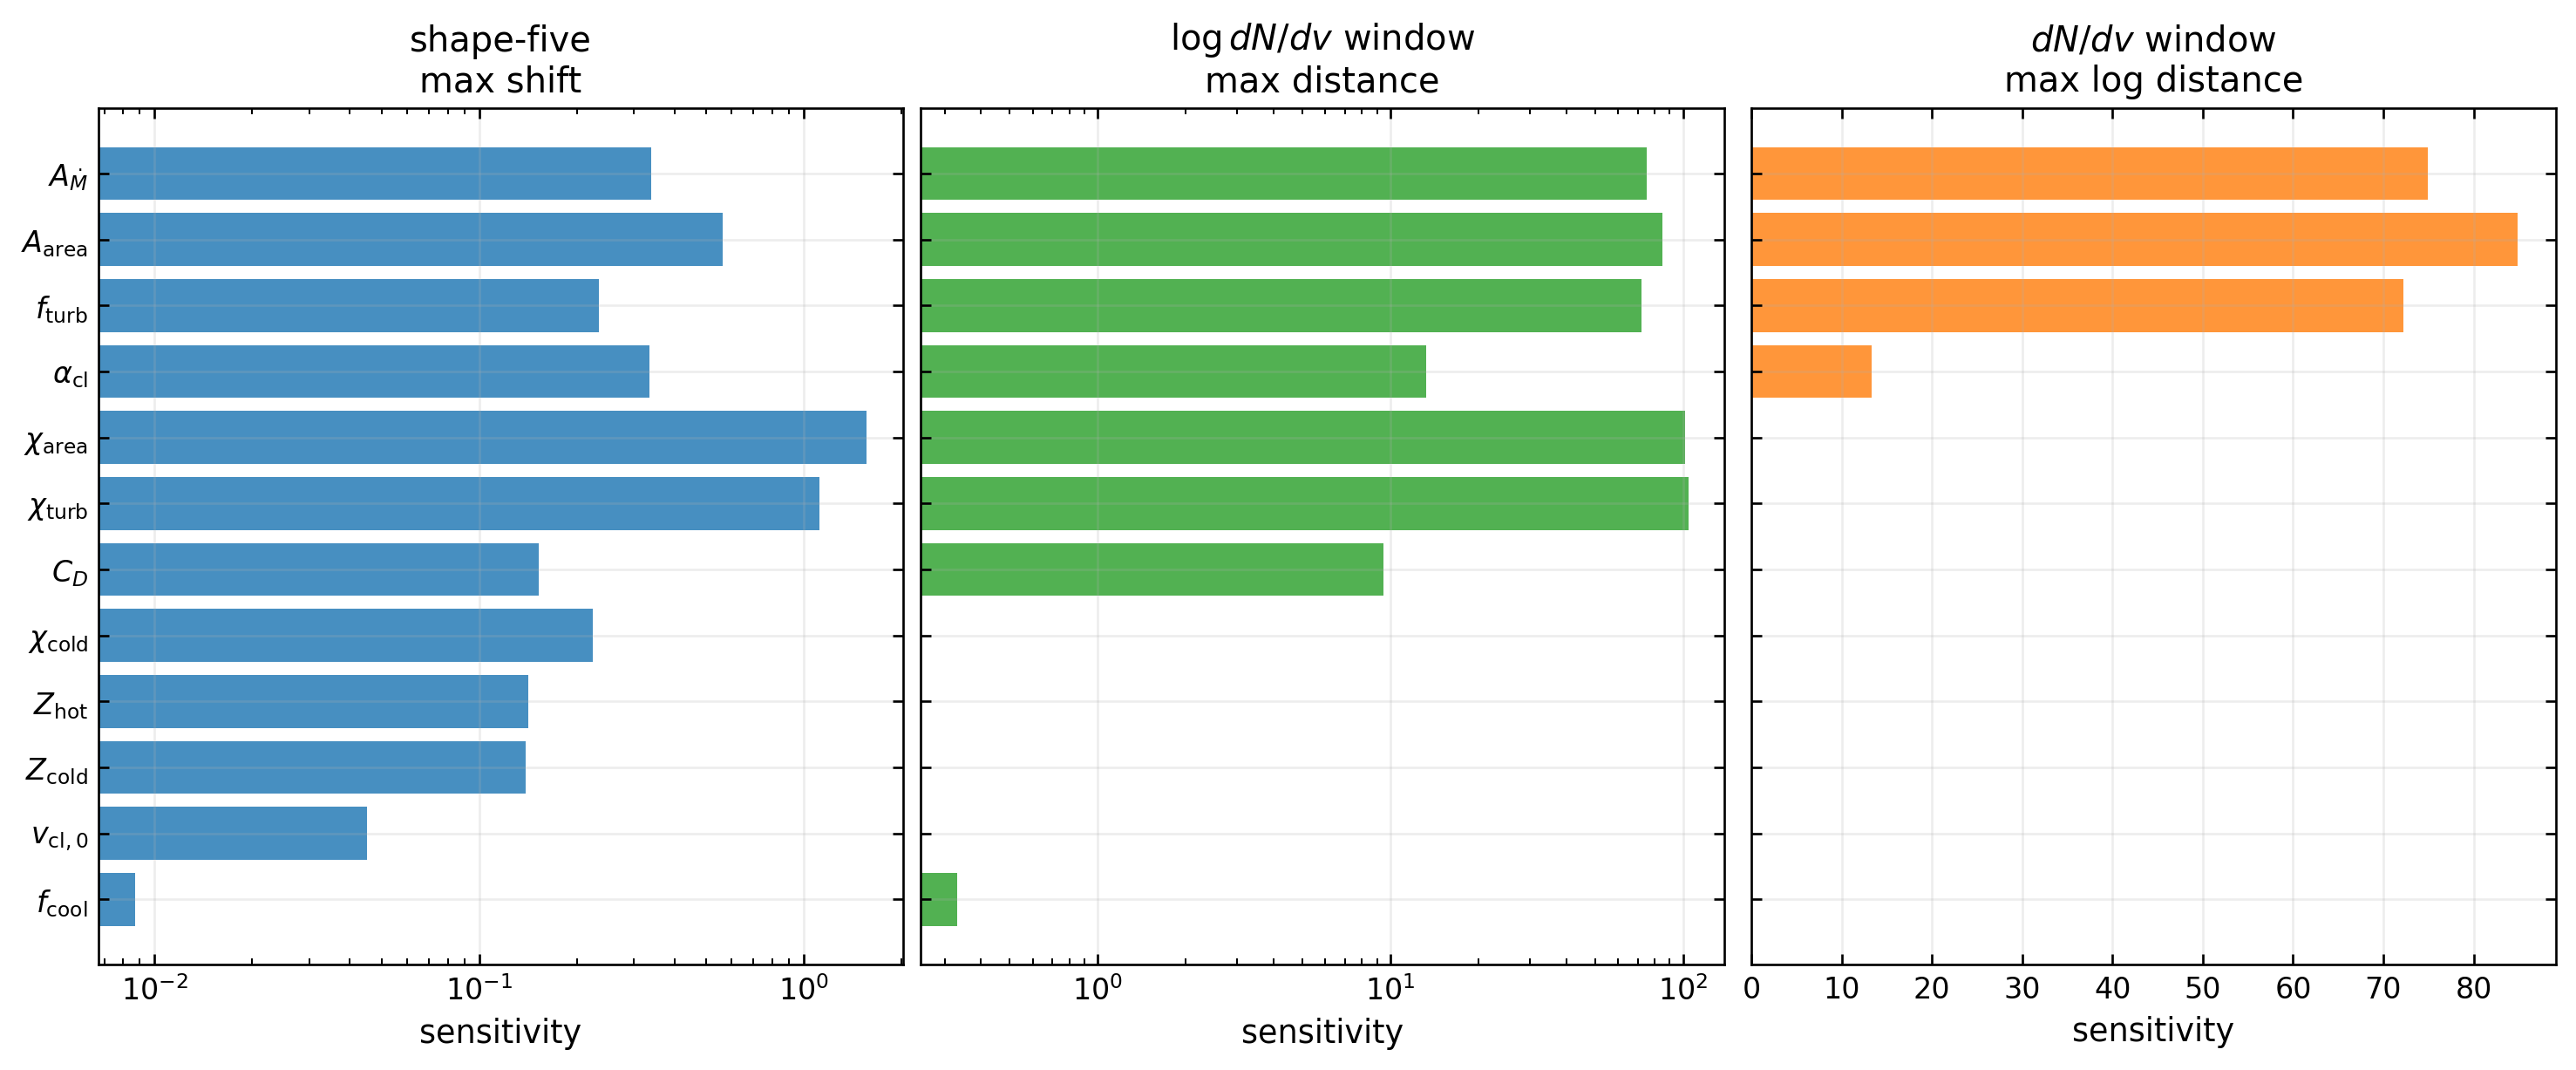
\includegraphics[width=\textwidth]{figures/trml_sensitivity_cross_case_ranking.png}
\caption{
Cross-case one-at-a-time sensitivity ranking for fixed cloud-wind and turbulent
radiative mixing-layer parameters.  The left panel shows the maximum shift in
the compact shape-five observable vector across the five synthetic truth cases.
The middle panel shows the maximum observed-window $\log dN/dv$ profile
distance for the profile-screen shortlist.  The right panel shows the analogous
linear-profile robustness check for the stable mixing-amplitude shortlist.  The
largest responses come from the $\chi$-dependent turbulent velocity and area
exponents and from effective mixing-amplitude parameters such as the
mass-exchange prefactor, geometric area factor, and $f_{\rm turb}$.  These
large shifts demonstrate that the microphysics matters for the forward model,
but they do not by themselves establish that the parameters are independently
inferable.
}
\label{fig:trml_sensitivity_cross_case_ranking}
\end{figure*}

Figure~\ref{fig:trml_sensitivity_cross_case_ranking} shows that the model is
not insensitive to the fixed microphysics.  The strongest compact-observable
responses come from the $\chi$-dependent area and turbulent-velocity exponents.
In the observed-window profile screen these same exponents can move the log
profile by tens of likelihood-scale units.  The effective amplitude-like
parameters, especially the mass-exchange prefactor, geometric area factor, and
$f_{\rm turb}$, also move both the compact summaries and the profile shape.  By
contrast, the global hot cooling multiplier is nearly inert in this reduced
screen, and the metallicity variations have lower leverage than the mixing and
turbulence parameters.

\begin{figure*}[t]
\centering
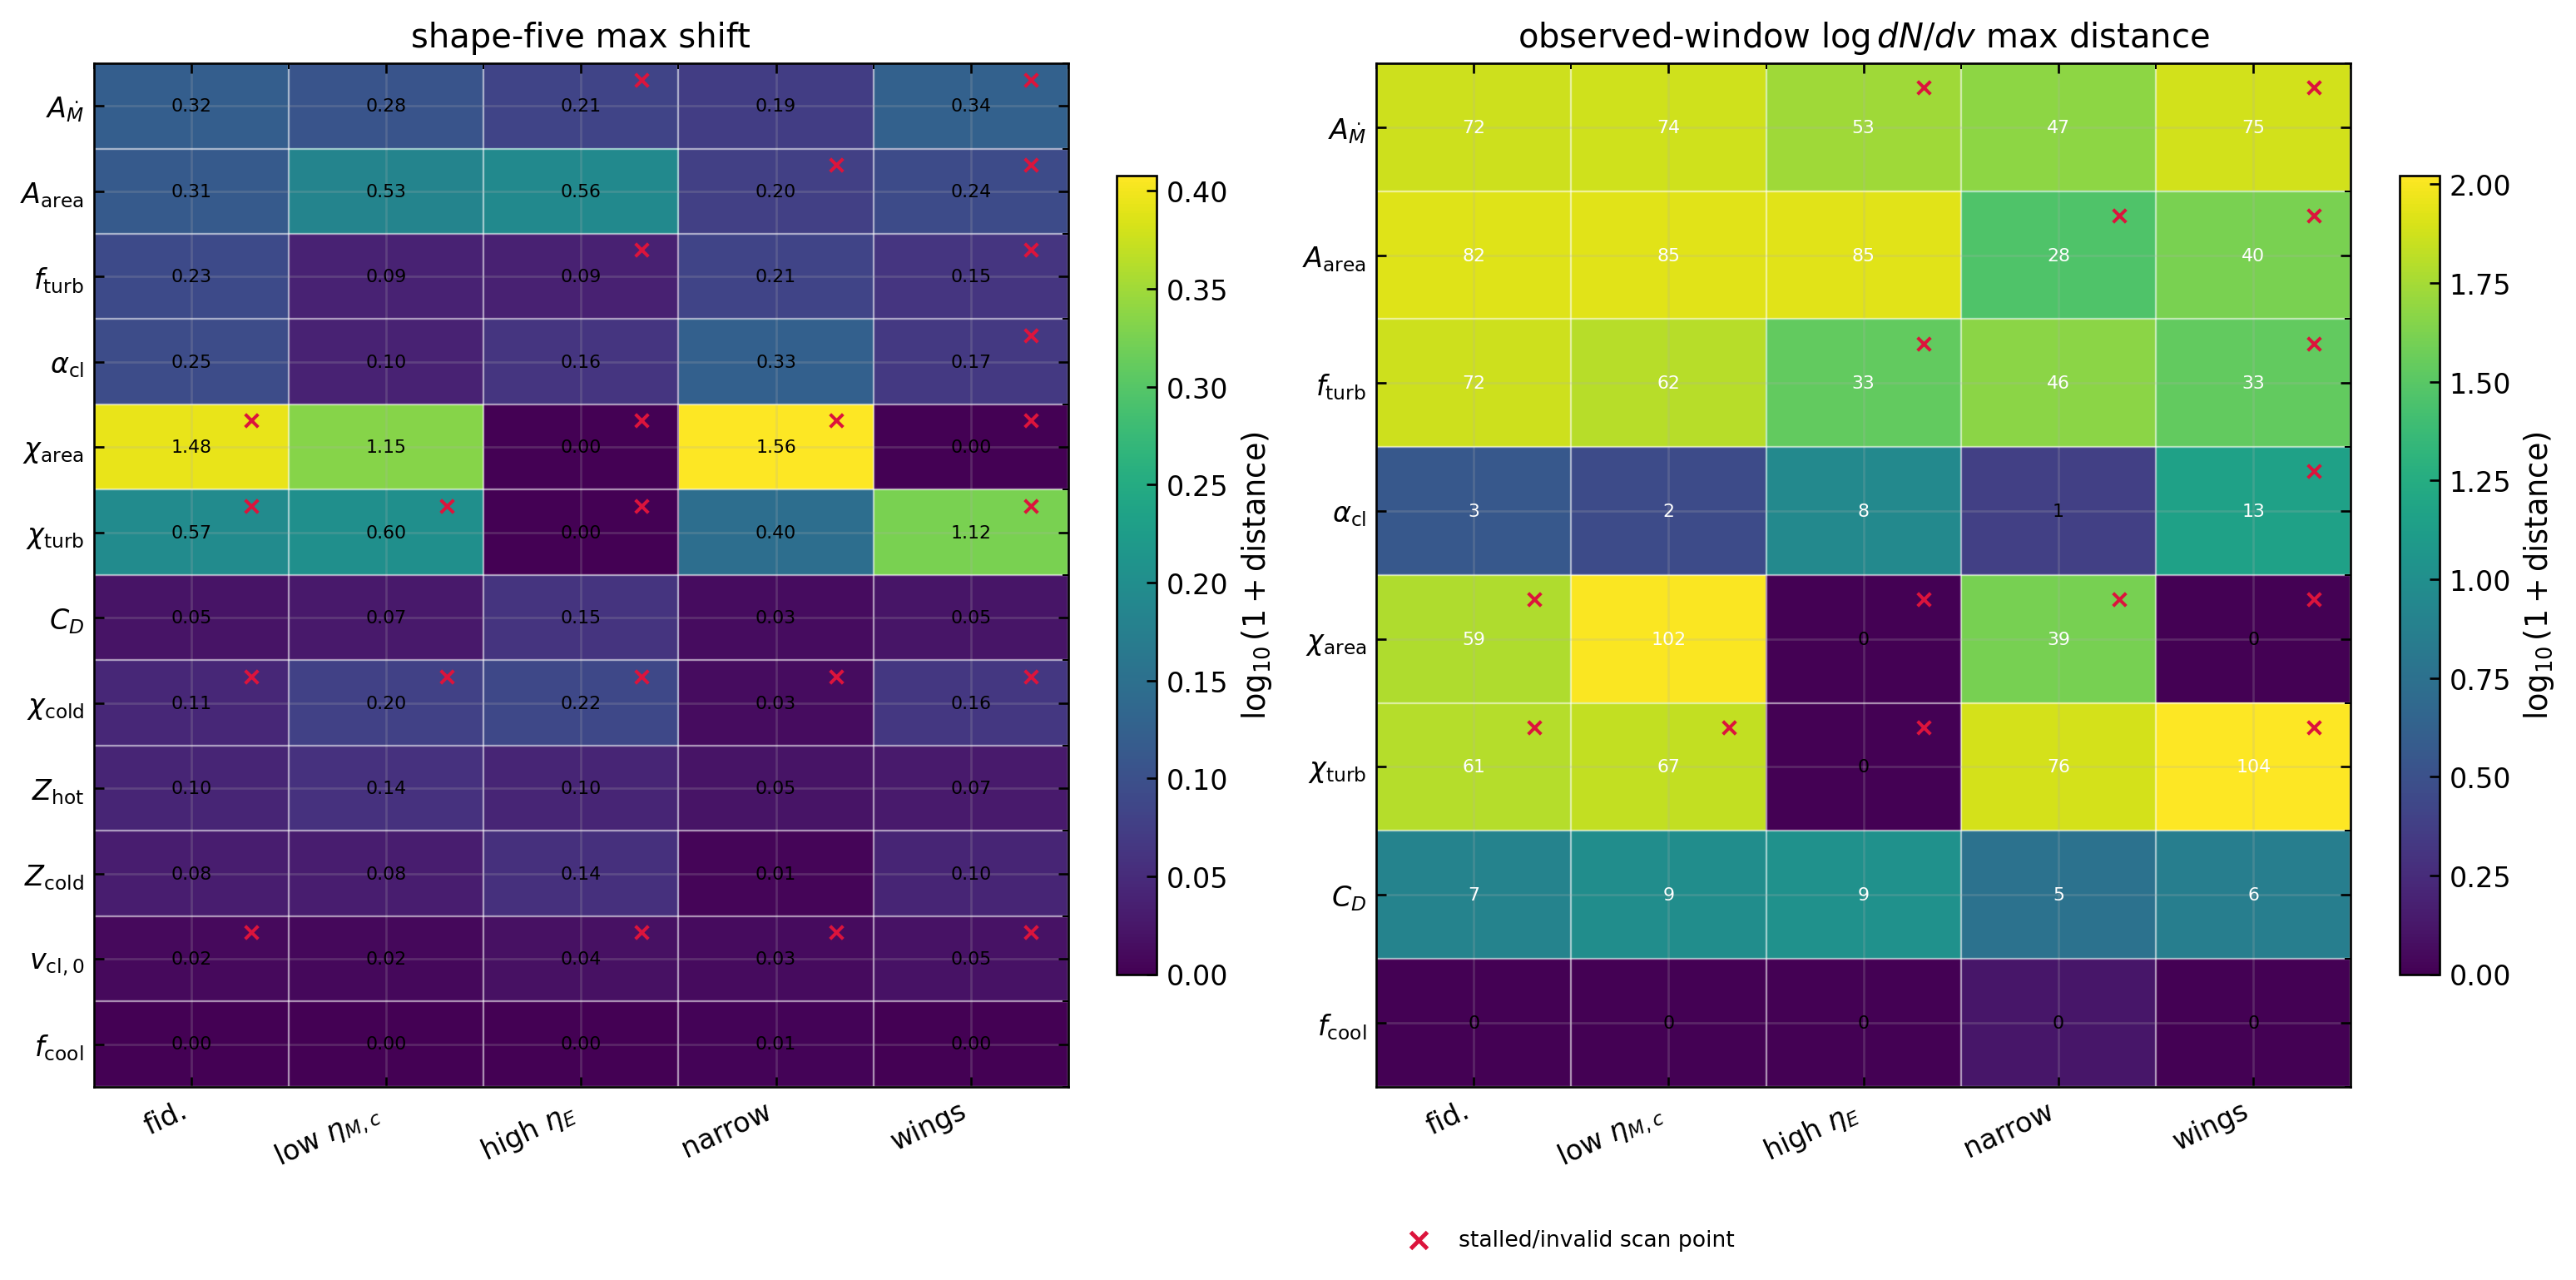
\includegraphics[width=\textwidth]{figures/trml_sensitivity_per_case_heatmap.png}
\caption{
Per-case sensitivity and validity.  The left panel shows the maximum
shape-five shift for every scanned parameter and truth case.  The right panel
shows the observed-window $\log dN/dv$ profile distance for the profile-screen
shortlist.  Cell colors use $\log_{10}(1+\mathrm{distance})$; the overplotted
numbers give the untransformed distances.  Red crosses mark truth-case and
parameter combinations for which at least one scan point stalled or became
invalid.  The heatmap shows that the conclusion is not driven solely by the
\texttt{strong\_wings} stress case: mixing-amplitude and $\chi$-exponent
directions have leverage across ordinary and high-energy cases, while the
validity problems concentrate in the same directions that most strongly alter
the wind.
}
\label{fig:trml_sensitivity_per_case_heatmap}
\end{figure*}

The important caveat is validity.  The high-leverage exponent directions often
move the model into stalled-wind regimes.  For example, increasing the cooling
area exponent or changing the turbulent-velocity exponent can cause several
truth cases to stall before the observable radius.  Stronger mixing-amplitude
settings also fail in the high-specific-energy cases: large values of the
mass-exchange prefactor or $f_{\rm turb}$ can stall
\texttt{low\_eta\_m\_high\_eta\_e} or \texttt{strong\_wings}.  This is a
physically meaningful result.  These parameter values produce winds that do not
reach the observable radius, and the stalled-wind inference policy reports them
as finite low-probability forward-model outcomes.  But they are not clean first
directions for expanded inference.

Figure~\ref{fig:trml_sensitivity_per_case_heatmap} also clarifies the role of
the \texttt{strong\_wings} case.  That case remains a deliberately difficult
stress test, but it is not the sole source of the result.  The mass-exchange
prefactor, geometric area factor, and $f_{\rm turb}$ move the observed-window
profile in the fiducial and low-cold-loading cases as well as in the high-energy
cases.  The $\chi$-dependent exponents are even more global: one sign of the
perturbation can suppress mixing enough to remove the wings, while the other
can over-couple the phases and stall the wind.  Physically, these parameters
regulate how rapidly cold material exchanges mass, momentum, and energy with
the hot flow.  When the coupling is too strong, the hot phase can lose enough
specific energy to fail before $6\,{\rm kpc}$; when it is weaker, the cool
material survives to different velocities and changes the line-profile shape.
That is exactly the microphysics we eventually want to understand, but it is
not yet a stable fourth inference coordinate.

\begin{figure*}[t]
\centering
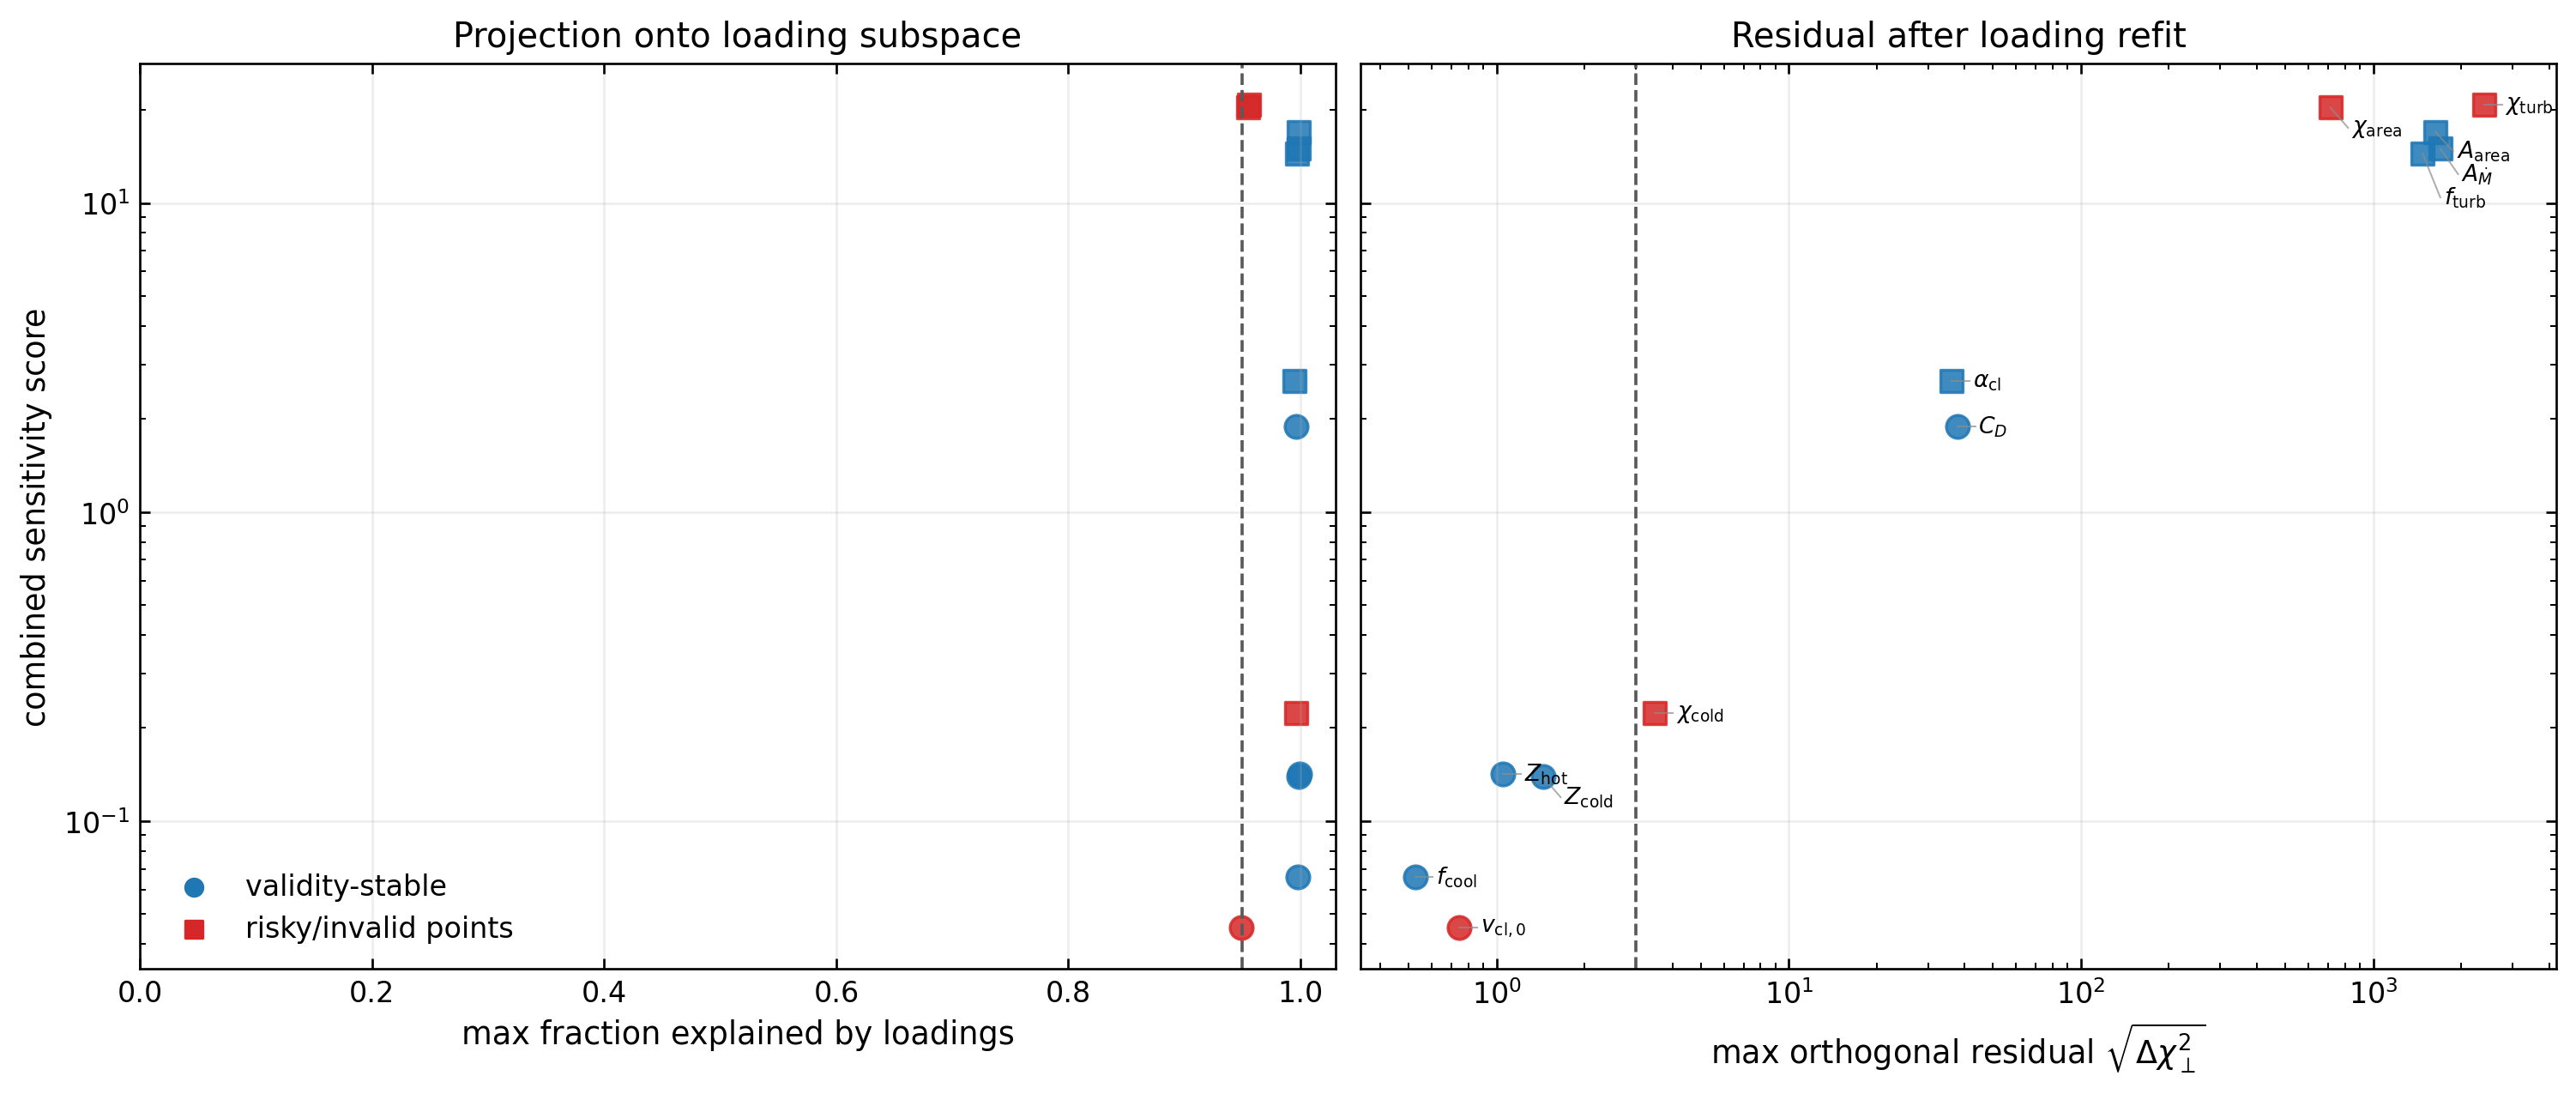
\includegraphics[width=\textwidth]{figures/trml_sensitivity_leverage_degeneracy.png}
\caption{
Observable leverage versus covariance-whitened loading-subspace projection.
The left panel shows the maximum fraction of the microphysics-induced
observable displacement that can be fit by the best linear combination of
finite-difference changes in $\eta_M$, $\eta_{M,\rm cold}$, and $\eta_E$; the
dashed line marks 0.95.  The right panel shows the remaining orthogonal
residual, $\sqrt{\Delta\chi^2_\perp}$, after that loading refit; the dashed line
marks a residual of 3.  Blue points are validity-stable across the scanned
range; red squares have repeated stalled or invalid scan points.  The
high-leverage directions are mostly loading-like in their leading response, but
their observed-window profile shifts leave large non-loading residuals under
the adopted covariance.
}
\label{fig:trml_sensitivity_leverage_degeneracy}
\end{figure*}

Figure~\ref{fig:trml_sensitivity_leverage_degeneracy} shows why this result does
not reduce to a simple yes-or-no degeneracy statement.  The leading response of
most high-leverage parameters is indeed close to the loading subspace: the
maximum explained fraction is typically $0.95$--$0.998$.  However, the profile
displacements are so large that the residual left after the best loading refit
can still be many likelihood sigma.  Thus the microphysics directions are
mostly loading-like, but not mathematically identical to loading changes.  This
is stronger evidence than the pairwise cosine test that profile data could
eventually help distinguish an effective mixing parameter from the three
loadings.

This does not mean the microphysics is unimportant.  It means that the present
observable set is not yet sufficient to infer a broad cloud-wind closure model.
The screen favors a narrow interpretation.  If an expanded parameter is tested
later, the most physically controlled first candidate is an effective mixing
amplitude, for example a multiplier on the mass-exchange prefactor.  Even that
candidate should use a restricted prior, because the high-amplitude end of the
scan produces stalled winds in the high-energy cases.  The drag coefficient is
validity-stable and has measurable profile leverage, but its overall response is
smaller than the mixing-amplitude directions and it is lower priority as a first
expansion.

The result would change in one of three ways.  First, a parameter could remain
high leverage while avoiding repeated stalled scan points over a physically
reasonable prior range.  Second, its observable displacement could become less
parallel to the loading directions, either because multiple objects are fit
jointly or because additional observables isolate the microphysics.  Third, a
restricted effective parameter such as $A_{\rm mix}$ could pass its own prior
predictive and synthetic-recovery gate.  None of those conditions is met by the
present screen.

We therefore stop short of adding a new inferred parameter at this stage.  The
Step~7 result is negative but useful: the forward model is sensitive to
cloud-wind microphysics, but the current three-parameter validation does not
support fitting a broad set of TRML closure knobs.  The next decision should
focus on a very restricted $A_{\rm mix}$ experiment with its own prior
predictive and synthetic-recovery gate, rather than a general expansion of the
closure model.

\clearpage
